\chapter{Approach, Methodology and Results}
\section{Approach}

The approach to enhancing network accuracy whilst preserving human aligned concepts, was formulated through a series of informal discussions with departmental colleagues and co-authors as noted in \cite{grangeXAISelfexplanatoryAI2022}. Consequently, both I and others, were already invested in the idea, so the decision to commit to the further utilisation of the existing model that had been researched and developed made logical sense. The decision to approach the project using this existing constrained sequential CBM and expert-rated data set \cite{grangeXAISelfexplanatoryAI2022} as a starting point provided me with the advantage of being able to meet the aims and objectives of the dissertation within the given time frame, without building a network from scratch.

The use of this model and subsequent dataset also had the distinct advantage of empirical evidence for the validity of the feature concepts in the research conducted by Nosofsky et al. (\cite{nosofskyDevelopmentFeaturespaceRepresentation2018}, \cite{miyatsuFeatureHighlightingEnhances2019}, \cite{sandersTrainingDeepNetworks2020})., The data set was also unique in its use of combining both \emph{soft}, information rich, scalar concepts (in this instance between 1 and 9), and \emph{harder} binary concepts (1 or 9). The reasoning for using a scale of 1-9 is rooted in the initial dataset of MDS co-ordinates from Nosofsky et al. It was, and remains, unclear if this a-typical method of rating feature concepts improves performance in comparison to other \emph{soft} CBM models, of which use probability ratings between 0-1. It is also worthy of noting that in previous iterations of the network (in the build up to \cite{grangeXAISelfexplanatoryAI2022})  that a model gradients function was used, penalising any feature concepts that were rated as -1 i.e.  not present. However this method of rating concepts was removed due to the analysis showing a reduction in the accuracy of classification and weak concept alignment. Evidence in the literature for improved classification accuracy when using \emph{soft} scalar concepts has been pointed to as a potential result of information \emph{leakage} \cite{havasiAddressingLeakageConcept2022a} i.e. soft concepts may be misrepresenting the data, and therefore muddying the interpretability of the model. Yet with binary concepts, despite being more truthful, they often penalise the accuracy of the classification. This has been hypothesised as a potential result of the lack of required concept features needed by the model. The discovery of this in the literature only served to strengthen my initial thoughts on the matter and concluded that it was a worthy avenue of research within this project. 

Amongst other proposals considered, was that of joint training through a combined loss function, akin to Koh et al. \cite{kohConceptBottleneckModels2020}. However, I believed there was a pressing need for a deeper understanding of what the existing sequential CBM model had learnt with regards to the validity of the concepts. This was further supported by claims from Margeloiu et al. \cite{margeloiuConceptBottleneckModels2021}  that joint CBMs have a tendency towards a low correlation of concept values, and that the benefits that may be had from intervention are in fact detrimental to performance.

The desire to understand more about the sequential CBM developed by Grange et al. and the concepts it had learnt, eventually fostered the novel idea that the weights and biases (\emph{w} + \emph{b}) learnt by the existing CBM \cite{grangeXAISelfexplanatoryAI2022} could be used to initialise a new CBM classifier. The decision to take this approach was based on the notion that by giving the network some additional degrees of freedom to learn, greater classification accuracy may be achieved (akin to that of a black box) whilst regaining the existing highly correlated expert feature values. Additionally, the appended hybrid network could serve as a tool for assessing the quality of the learnt expert feature values in the sequential bottleneck model via comparative correlation. In turn, allowing the user to intervene with the training data.

The framework of the approach adopted comprised of the following steps: 

\begin{itemize}
\item Utilisation of the model proposed by Grange at al. 2022 \cite{grangeXAISelfexplanatoryAI2022} as a foundational starting point

\item The development of an additional network classifier that employs the acquired knowledge embedded within the weights and biases of the previous CBM model \cite{grangeXAISelfexplanatoryAI2022}. Implementation in MATLAB \cite{MATLAB}, following the methodology of the previous model, will expedite development and subsequent data collection

\item Developing analytical tools with which to appraise the classification accuracy and concept alignment of the new hybrid classifier to that of the prior CBM and to the expert training data

\item Quantifying the effects on classification accuracy and concept alignment when using binary or continuous concept/feature ratings

\item Evaluating the impact on classification accuracy when removing a concept/feature with low correlation to the input dataset of human intelligible features

\item Investigating the outcomes on classification accuracy and concept alignment through the manipulation of network learning variables, such as the number of epochs, mini-batch size, and learning rate

\end{itemize}

Throughout the project an ongoing literature review was conducted in order to keep abreast of new developments in the field of XAI. The lack of clarity with regards to terminology in the domain was a considerable hindrance during the development of the initial sequential CBM \cite{grangeXAISelfexplanatoryAI2022}. As such it was essential that I made a continued effort to build a repository throughout the project to inform my decisions and prevent the replication of research already conducted in previous studies. I found many examples of post-hoc CBM methods (\cite{havasiAddressingLeakageConcept2022a}, \cite{yuksekgonulPosthocConceptBottleneck2022}, \cite{daneshjouSkinConSkinDisease2022}), and others that addressed the loss of concept clarity or “leakage” \cite{mahinpeiPromisesPitfallsBlackBox2021}, however I did not find evidence of the methodology as proposed in this work, being replicated elsewhere.

\section{Design and Implementation}

The development of the hybrid classifier network was completed in Matlab as planned. A snippet of the code can be see below:

\lstinputlisting[language=Matlab,firstline=559, lastline=605, caption= Matlab code for the Hybrid Network Classifier]{Code/networksAll.m}

The design developed continues the use of transfer learning as per \cite{grangeXAISelfexplanatoryAI2022}, taking in the 2048 features from ResNet50, with a 50\% dropout layer, in line with the previous CBM design. However, where the new hybrid classifier differs is in that the three fully connected layers are initialised with the weights and biases (\emph{w} + \emph{b}) learned from the constrained sequential CBM (see Figure ~\ref{fig:Hybrid classifier XAI&I}). The first fully connected layer consists of 256 nodes which are not allowed to learn (with a learning rate of $\eta$ = 0). In contrast, the subsequent fully connected layers, of 13 nodes in the concept layer and 10 nodes in the classification layer, are free to do so (with an initial learning rate of $\eta$ = 0.001). This flexibility in the model to deviate along only two of the feature layers (concept and classification layers), using the same number of nodes as per the previous CBM (except for the case of one experimental method of removing one concept, and subsequently one node in the concept layer), made it possible to evaluate the results against both the original CBM and the expert training data. This design ensured that the resultant concept features were prevented from straying too far outside of the bound of 1-9, as per the original training data.

One may view the hybrid classifier as an extension of a sequential CBM, due to the manner in which it relies upon the weights and biases of the preceding network classifier, thus in reference to the terminology used in the literature one could pertain that this model functions as a post-hoc sequential CBM.

\begin{figure}[H]
  \centering
    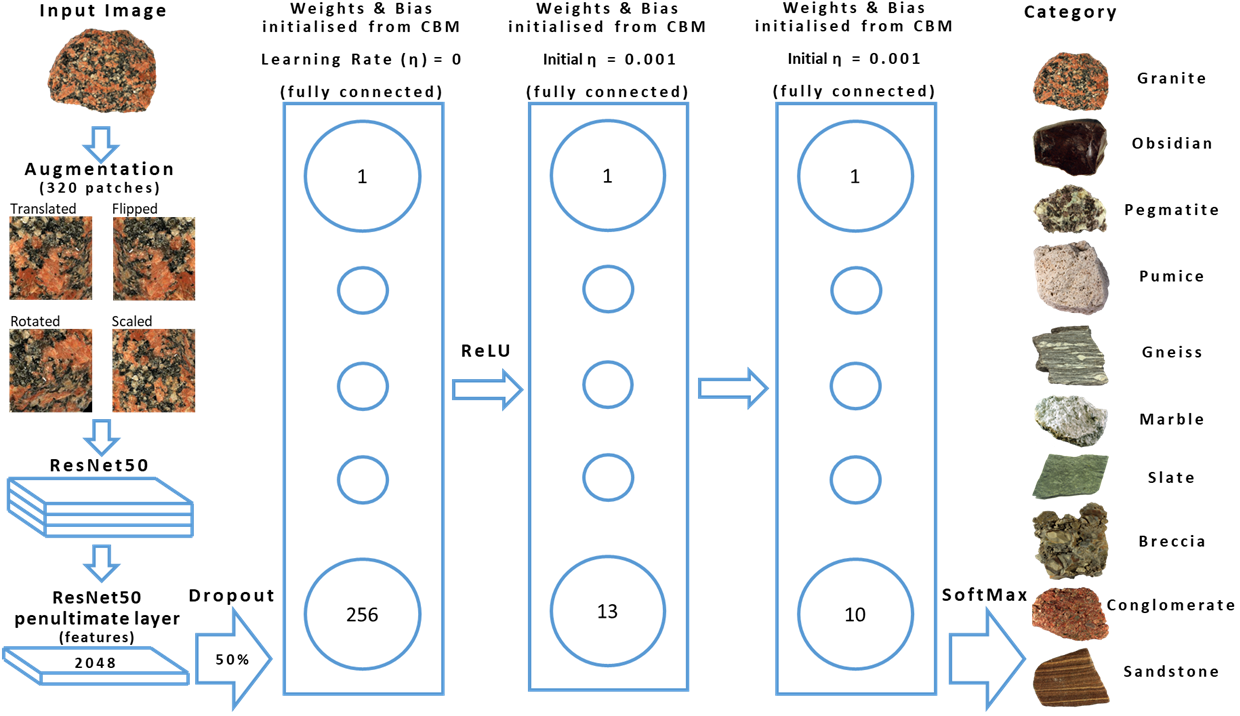
\includegraphics[width=\textwidth]{images/Hybrid Network Figure V2.png}
    \caption{The framework of the hybrid CBM classifier} \label{fig:Hybrid classifier XAI&I}
\end{figure}

Concurrently an partially feature constrained black-box model was developed akin to that in \cite{grangeXAISelfexplanatoryAI2022} (see figure \ref{fig:Networks 1-3 XAI&I}). The number of feature nodes was set to 13 in order to enable a a fair comparison to that of the hybrid CBM.

For one to achieve a sufficient set of data to equate to fair analysis of variance, the code was automated (see code ~\ref{lst:Automating 12 runs of 12 sets of validation images}) to complete 12 runs of 12 alternating validation sets. The output of each of which required collation and manipulation for analysis of accuracy, and concept alignment between each of the networks and that of the original set of expert ratings (an example of the training data used for Granite can be seen her \ref{An Example of 13 Expert Feature Ratings for Granite - As Used for Training})

Analysis of the immense collation of data from each permutation and manipulation of the models required the development of a plethora of Jupyter notebooks insights it held(\ref{fig:Code for the Analysis and Visualisation of Pearson's Correlation Co-Efficient of Feature Ratings Between Expert Feature Ratings, Sequential CBM and Hybrid Classifier CBM}, \ref{fig:Means and Standard Error of the Mean (SEM) Between Validation Sets - Analysis and Visualisation coded in Jupyter Notebooks using Plotly for Visualisation}, \ref{fig:Comparing the Accuracy of Rock Predictions - Hybrid - Continuous vs Binary Crystal Ratings}), with which manipulate the data and visualise it using the Python library \emph{Plotly} \cite{plotly} (see Appendix subsection: \ref{Data Visualisations}). This served as in order to expedite insight at a far greater pace.

\newpage
\section{Results}

My initial investigation took the form of manipulating training variables such as the number of epochs, mini-batch size and learning rate.

Through the analysis of training data visualisations it was clear that  validation accuracy of the original CBM was diverging from the training accuracy as I increased the number of epochs, a sign of the over-fitting the data. As such, the correlation of the output features with that of expert features was not negatively effected, with insignificant variance. The opposite was true when reducing the number of epochs, with a sweet spot between 175-200. As such, I decided to stick to the existing use of 200 epochs, as this made it simpler when comparing to previous iterations.

The manipulation of learning rate was of little benefit to the existing CBM model, reducing performance when the number of epochs was increased, yet was not significant enough to warrant further exploration. I believe this in part to be the benefit of the \emph{Adam Optimiser} \cite{Kingma2014Dec}, of which upon research appears to be a common effect due to its inherent ability to self-tune. Therefore I concluded that leave the learning rate at $10^{-3}$ (0.001) was adequate.

The manipulation of mini-batch size is another method typically used to prevent validation accuracy from diverging from training accuracy. I explored the use of reducing the size down to 256, which appeared to decrease divergence, however was of no benefit to performance. Upon further reading, many note that in some instance some over-fitting can be beneficial to a model, and as I was going to explore the benefits of appending the hybrid classifier, I returned to using a mini-batch size of 1024. 

For further analysis, some of the results of these manipulations can be seen in the appendix \ref{Feature Correlations - 13 Features - Continuous Scalar Crystal Rating 1 Run of 12 Alternating Validation Sets - Part 2}.

Despite there being no grand finding from the manipulation of training variables, the results from the use of the hybrid network were however successful, with the aim of achieving an improved accuracy in classification that is on par to that of a black-box model. The 13 feature hybrid CBM classifier achieved a classification accuracy of 87.8\% (SD 0.58\%), an improvement of 1.27\% in comparison to the partially feature-constrained model of 86.53\% (SD 4.39\%) and unconstrained network’s performance (mean 86.8\%, SD 0.8\%). Interestingly the 12 feature network, with the weakly correlated n the concept of \emph{Brightness Heterogeneity} removed (Continuous crystal rating CBM network \emph{r} = 0.43, Hybrid CBM network \emph{r} = 0.3, Binary crystal rating CBM network \emph{r} = 0.45, Hybrid CBM network \emph{r} = 0.27, \ref{Data Visualisations}) performed well achieving a higher classification accuracy mean of 88.36\% yet with a larger standard deviation of the means of 3.41\%.


\scriptsize
\begin{longtable}[c]{@{}llllll@{}}
 &
  \multicolumn{2}{c}{\textbf{13 Features}} &
  \multicolumn{1}{c}{\textbf{Unconstrained 13}} &
  \multicolumn{2}{c}{\textbf{12 Features}} \\
  \toprule
\endfirsthead
%
\multicolumn{6}{c}%
{{\bfseries Table \thetable\ continued from previous page}} \\
\endhead
%
 &
  \cellcolor[HTML]{E2EFDA}\textbf{Continuous} &
  \cellcolor[HTML]{FFE699}\textbf{Binary Crystal} &
  \cellcolor[HTML]{D9E1F2}\textbf{} &
  \cellcolor[HTML]{E2EFDA}\textbf{Continuous} &
  \cellcolor[HTML]{FFE699}\textbf{Binary Crystal} \\
  \toprule
\textbf{Runs/Val Sets} &
  \cellcolor[HTML]{FCE4D6}12/12 &
  \cellcolor[HTML]{FCE4D6}12/12 &
  \cellcolor[HTML]{FCE4D6}12/12 &
  \cellcolor[HTML]{FCE4D6}12/12 &
  \cellcolor[HTML]{FCE4D6}12/12 \\
  \toprule
\rowcolor[HTML]{E7E6E6} 
\textbf{C2} &
   &
   &
   &
   &
   \\
\textbf{Epochs} &
  \cellcolor[HTML]{E2EFDA}200 &
  \cellcolor[HTML]{FFE699}200 &
  \cellcolor[HTML]{D9E1F2}200 &
  \cellcolor[HTML]{E2EFDA}200 &
  \cellcolor[HTML]{FFE699}200 \\
\textbf{Learning Rate} &
  \cellcolor[HTML]{E2EFDA}{\color[HTML]{202124} 0.001} &
  \cellcolor[HTML]{FFE699}{\color[HTML]{202124} 0.001} &
  \cellcolor[HTML]{D9E1F2}{\color[HTML]{202124} 0.001} &
  \cellcolor[HTML]{E2EFDA}{\color[HTML]{202124} 0.001} &
  \cellcolor[HTML]{FFE699}{\color[HTML]{202124} 0.001} \\
\textbf{Learning Rate} &
  \cellcolor[HTML]{E2EFDA}{\color[HTML]{202124} 10\textasciicircum{}-3} &
  \cellcolor[HTML]{FFE699}{\color[HTML]{202124} 10\textasciicircum{}-3} &
  \cellcolor[HTML]{D9E1F2}{\color[HTML]{202124} 10\textasciicircum{}-3} &
  \cellcolor[HTML]{E2EFDA}{\color[HTML]{202124} 10\textasciicircum{}-3} &
  \cellcolor[HTML]{FFE699}{\color[HTML]{202124} 10\textasciicircum{}-3} \\
\textbf{Minibatch Size} &
  \cellcolor[HTML]{E2EFDA}{\color[HTML]{202124} 1024} &
  \cellcolor[HTML]{FFE699}{\color[HTML]{202124} 1024} &
  \cellcolor[HTML]{D9E1F2}{\color[HTML]{202124} 1024} &
  \cellcolor[HTML]{E2EFDA}{\color[HTML]{202124} 1024} &
  \cellcolor[HTML]{FFE699}{\color[HTML]{202124} 1024} \\
\textbf{Accuracy Mean - Val Set} &
  \cellcolor[HTML]{E2EFDA}83.66\% &
  \cellcolor[HTML]{FFE699}84.63\% &
  \cellcolor[HTML]{D9E1F2}\textbf{87.15\%} &
  \cellcolor[HTML]{E2EFDA}82.25\% &
  \cellcolor[HTML]{FFE699}82.48\% \\
\textbf{SEM - Val Set} &
  \cellcolor[HTML]{E2EFDA}0.52\% &
  \cellcolor[HTML]{FFE699}0.53\% &
  \cellcolor[HTML]{D9E1F2}0.83\% &
  \cellcolor[HTML]{E2EFDA}0.52\% &
  \cellcolor[HTML]{FFE699}0.57\% \\
\textbf{Accuracy Mean - Run Set} &
  \cellcolor[HTML]{E2EFDA}83.66\% &
  \cellcolor[HTML]{FFE699}84.63\% &
  \cellcolor[HTML]{D9E1F2}\textbf{86.53\%} &
  \cellcolor[HTML]{E2EFDA}82.25\% &
  \cellcolor[HTML]{FFE699}82.48\% \\
\textbf{STD of Means - Run Set} &
  \cellcolor[HTML]{E2EFDA}0.57\% &
  \cellcolor[HTML]{FFE699}\textbf{4.03\%} &
  \cellcolor[HTML]{D9E1F2}\textbf{4.39\%} &
  \cellcolor[HTML]{E2EFDA}\textbf{3.57\%} &
  \cellcolor[HTML]{FFE699}2.79\% \\
\textbf{SEM - Run Set} &
  \cellcolor[HTML]{E2EFDA}0.16\% &
  \cellcolor[HTML]{FFE699}1.16\% &
  \cellcolor[HTML]{D9E1F2}1.27\% &
  \cellcolor[HTML]{E2EFDA}1.03\% &
  \cellcolor[HTML]{FFE699}0.80\% \\
  \toprule
\rowcolor[HTML]{E7E6E6} 
\textbf{Hybrid} &
   &
   &
   &
   &
   \\
   
\textbf{Epochs} &
  \cellcolor[HTML]{E2EFDA}50 &
  \cellcolor[HTML]{FFE699}50 &
  \cellcolor[HTML]{D9E1F2} &
  \cellcolor[HTML]{E2EFDA}50 &
  \cellcolor[HTML]{FFE699}50 \\
\textbf{Learning Rate} &
  \cellcolor[HTML]{E2EFDA}{\color[HTML]{202124} 0.001} &
  \cellcolor[HTML]{FFE699}{\color[HTML]{202124} 0.001} &
  \cellcolor[HTML]{D9E1F2}{\color[HTML]{202124} } &
  \cellcolor[HTML]{E2EFDA}{\color[HTML]{202124} 0.001} &
  \cellcolor[HTML]{FFE699}{\color[HTML]{202124} 0.001} \\
\textbf{Learning Rate} &
  \cellcolor[HTML]{E2EFDA}{\color[HTML]{202124} 10\textasciicircum{}-3} &
  \cellcolor[HTML]{FFE699}{\color[HTML]{202124} 10\textasciicircum{}-3} &
  \cellcolor[HTML]{D9E1F2}{\color[HTML]{202124} } &
  \cellcolor[HTML]{E2EFDA}{\color[HTML]{202124} 10\textasciicircum{}-3} &
  \cellcolor[HTML]{FFE699}{\color[HTML]{202124} 10\textasciicircum{}-3} \\
\textbf{Minibatch Size} &
  \cellcolor[HTML]{E2EFDA}1024 &
  \cellcolor[HTML]{FFE699}1024 &
  \cellcolor[HTML]{D9E1F2} &
  \cellcolor[HTML]{E2EFDA}1024 &
  \cellcolor[HTML]{FFE699}1024 \\
\textbf{Accuracy Mean -  Val Set} &
  \cellcolor[HTML]{E2EFDA}87.80\% &
  \cellcolor[HTML]{FFE699}87.59\% &
  \cellcolor[HTML]{D9E1F2} &
  \cellcolor[HTML]{E2EFDA}87.55\% &
  \cellcolor[HTML]{FFE699}\textbf{88.36\%} \\
\textbf{SEM - Val Set} &
  \cellcolor[HTML]{E2EFDA}0.68\% &
  \cellcolor[HTML]{FFE699}0.70\% &
  \cellcolor[HTML]{D9E1F2} &
  \cellcolor[HTML]{E2EFDA}0.65\% &
  \cellcolor[HTML]{FFE699}\textbf{0.62\%} \\
\textbf{Accuracy Mean - Run Set} &
  \cellcolor[HTML]{E2EFDA}\textbf{87.80\%} &
  \cellcolor[HTML]{FFE699}87.59\% &
  \cellcolor[HTML]{D9E1F2} &
  \cellcolor[HTML]{E2EFDA}87.55\% &
  \cellcolor[HTML]{FFE699}\textbf{88.36\%} \\
\textbf{STD of Means - Run Set} &
  \cellcolor[HTML]{E2EFDA}0.58\% &
  \cellcolor[HTML]{FFE699}\textbf{2.94\%} &
  \cellcolor[HTML]{D9E1F2}\textbf{} &
  \cellcolor[HTML]{E2EFDA}3.43\% &
  \cellcolor[HTML]{FFE699}\textbf{3.41\%} \\
\textbf{SEM - Run Set} &
  \cellcolor[HTML]{E2EFDA}0.17\% &
  \cellcolor[HTML]{FFE699}0.85\% &
  \cellcolor[HTML]{D9E1F2} &
  \cellcolor[HTML]{E2EFDA}0.99\% &
  \cellcolor[HTML]{FFE699}0.98\%
  \\
\caption{Classification accuracy ratings comparing network variables. The first two columns use 13 expert feature ratings for training and compare implications of using continuous or binary ratings for the presence of crystals. The "13 Unconstrained" column represents a black-box model, limited only by the constraint of using a layer of 13 nodes prior to classification. The last two columns use 12 expert feature ratings, with the most weakly correlated feature "Brightness Heterogeneity" removed. A comparison is also drawn as to the implications of using continuous or binary ratings for the presence of crystals.}
\label{Classification accuracy ratings comparing network variables}\\
\end{longtable}

\normalsize